%UNIT 1: QUALITATIVE AND GRAPHICAL APPROACHES
% Is first part of original 01.tex
%%%%%%%%%%%%%%%%%%%%%%%%%%%
%%%% Put the following at the top of each .tex file  %
\pagestyle{fancy}
\renewcommand{\theUnit}{1}
\ifthenelse{\isundefined{\UnitPageNumbers}}{}{\setcounter{page}{1}}
\rhead{Carlton and Devore Chapter \theUnit: Introduction to Probability}
\lhead{Math 3382: Statistical Theory}
%\lhead{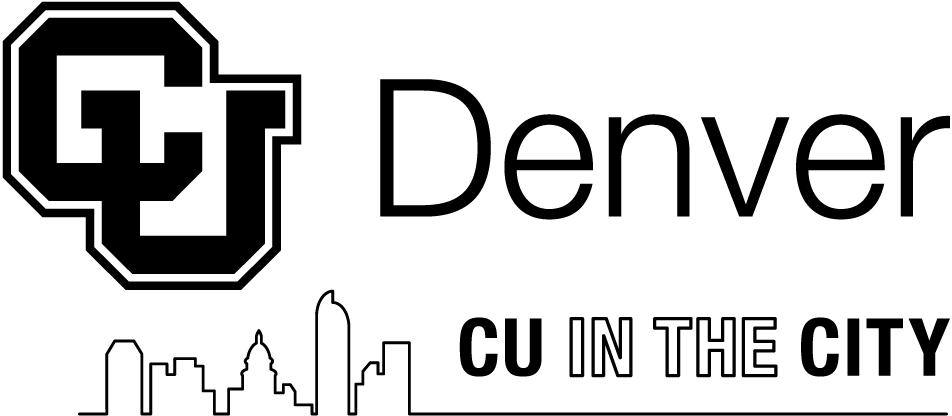
\includegraphics[width=1.25cm]{CUDenver-Logo.png}}
\rfoot{\mypage}
\cfoot{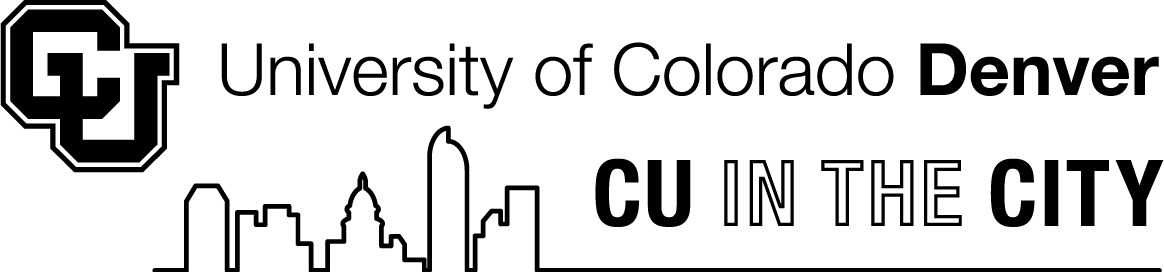
\includegraphics[width=2.25cm]{CUDenver-Logo-coverpage.png}}
\lfoot{Adam Spiegler}
\fancypagestyle{firstfooter}{\footskip = 50pt}
\renewcommand{\footrulewidth}{.4pt}
%%%%%%%%%%%%%%%%%%%%%%%%%%%
\vspace*{-20pt} \thispagestyle{firstfooter}
\pagebegin{Introduction to Probability}



%\pagebegin{Let's Make a Deal!}

%\begin{center}
%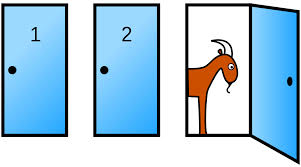
\includegraphics[width=3in]{03/03-montyhall.jpg}
%\end{center}
%\bs



%In the September 9, 1990 issue of \textit{Parade} magazine, the columnist Marilyn vos Savant responded to this letter:

%\begin{quotation}
%\textit{Suppose you’re on a game show, and you’re given the choice of three doors. Behind one door is a car, behind the others, goats. You pick a door, say number 1, and the host, who knows what’s behind the doors, opens another door, say number 3, which has a goat. He says to you, ``Do you want to pick door number 2?'' Is it to your advantage to switch your choice of doors?}
%\end{quotation}
%\hfill --Craig. F. Whitaker in Columbia, MD \bs

%The letter roughly describes a situation faced by contestants on the 1970’s game show Let’s Make a Deal, hosted by Monty Hall and Carol Merrill.


%\bb
%\ii After the host opens door 3, what is the best strategy: change doors or trust your initial choice? Play online and see how your strategy works:   \href{http://www.rossmanchance.com/applets/MontyHall/Monty04.html}{\underline{http://www.rossmanchance.com/applets/MontyHall/Monty04.html}}\label{playgame} \vfill

%\ii Rather than using simulations as in \ref{playgame}, give theoretical argument for why one strategy might be better than the other.\label{theorygame} \vfill
%\ee

%\clearpage

\bbox
\begin{definition}\label{def:ind}
 \ 
\bi 
%\ii A \textbf{statistical experiment or observation} is any random activity that results in a definite outcome.
\ii The \textbf{\alert{sample space}} $\Omega$ is the set of all possible outcomes of an experiment.
\ii An \textbf{\alert{outcome}} $\omega$, is a result from an experiment or observation.
\ii An \textbf{\alert{event}}, $A$, is a collection of one or more outcomes from an experiment or observation.
\ei
\end{definition}
\ebox

\bb
\ii In the 1970s, research\footnote{\href{www.laskerfoundation.org/rprimers/sommer/saving1.htm}{www.laskerfoundation.org/rprimers/sommer/saving1.htm} and \textit{Introduction to the Practice of Statistics}, 4th en, by David Moore, George. McCabe}  by Alfred Sommer on vitamin A and night blindness suggested that vitamin A also reduced childhood death rates. Children were randomly assigned to two groups, one group took a vitamin A pill every day, and children in the other group were given a \alert{placebo} (a pill that had no vitamin A). Below is a \colorb{two-way table} displaying the results of Sommer’s research.

\begin{center}
\begin{tabular}{l||c|c||c}
 & Vitamin A & No Vitamin A & Total \\
 \hline
 Died & 101 & 130 & 231 \\
 Lived & $12,\!890$ & $12,\!079$ & $24,\!969$\\
 \hline
 Total & $12,\!991$ & $12,\!209$ & $25\!,200$
 \end{tabular}
 \end{center}

\bb
\ii What is the probability that a randomly selected child in the study:
\bb
\ii  Died? \vfill
\ii Received the treatment, vitamin A? \vfill
%\ii Received a placebo, no vitamin A? \vfill
\ii Received vitamin A and died? \vfill
\ii Received vitamin A or died? \vfill
\ii Died given that they received vitamin A? \vfill
%\ii Died given that they did not receive vitamin A? \vfill
\ee
\ii Based on the data from this experiment, do you believe researchers can claim vitamin A decreases child mortality rates? \vfill
\ee
\ee

%\ii With how quickly new variants of COVID-19 develop and can potentially spread across the world, it is important to focus vaccinations efforts across the world. Below is a screenshot on August 28, 2021 from Our World in Data\footnote{\href{https://ourworldindata.org/covid-vaccinations}{https://ourworldindata.org/covid-vaccinations}}:

%\begin{center}
%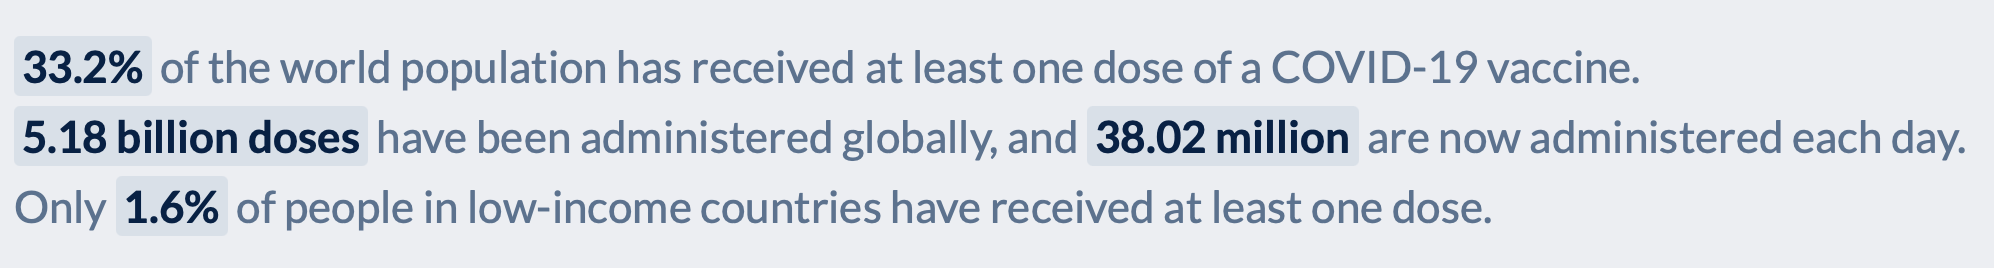
\includegraphics[width=0.85\tw]{03/fig-our-world-in-data.png}
%\end{center}

%Totals from Our World in Data are summarized in the table below, where the number of people is given in millions.

%\begin{tabular}{|l||c|c|c|c|c|c||c|}
%\hline
% & Africa & Asia & Australia & Europe & No. America & So. America & World\\
%\hline
%Full or Partial Vax & $65$ & $1,\!590$ & $12$ & $400$ & $316$ & $233$ & $2,\!616$\\
%Total Population & $1,\!370$ & $4,\!680$ & $26$ & $748$ & $597$ & $434$ & $7,\!855$\\
%\hline
%\end{tabular}

%\bb
%\ii What is the probability that a randomly selected person in the world is from Asia?
%\ii What is the probability that a randomly selected person in the world has received at least one vaccine dose?
%\ii What is the probability that a randomly selected person in the world is from Asia and received at least one vaccine does?
%\ii As of Aug, 28 2021, $1.59$ billion people in Asia had received at least one vaccine dose compared to $233$ million people in South America. Does this imply that Asia has done a better job at vaccinations compared to South America? Why or why not?
%\ee
%\ee

\clearpage

\pagebegin{Simple and Compound Probabilities}

\bbox
Let $A$ and $B$ denote two events in sample space $\Omega$, then
\bi
\ii $P(A)$ is the probability that event $A$ occurs.
\ii $P(A^C) = P(\bar{A}) = P(A')$ is the probability that \alert{event $A$ does NOT occur}.\\ The notation \alert{$A^C$, $\bar{A}$, or $A'$} are used to denote the \textbf{\alert{complement}} of $A$.
\ii \alert{$P(A \cap B)$} is the probability that events $A$ \textbf{\alert{and}} $B$ both occur.
\ii \alert{$P(A \cup B)$} is the probability that either event $A$ \alert{or} event $B$ occurs.
\ii \alert{$P(B \big| A )$} is the \textbf{\alert{conditional probability}} that event $B$ occurs \textbf{\alert{given that}} event $A$ occurs.
\ii \alert{$P(A - B)$} is the probability that event A occurs and event B does not occur.
\ei
\ebox


%\pagebegin{Set Notation}

%\bbox
%\begin{center}
%\begin{tabular}{|l|l|}
%\hline
%$\Omega$ & Sample space \\
%\hline
%$\omega$ & Outcome (single point or element in $\Omega$) \\
%\hline
%$A$ & An event (subset of $\Omega$) \\
%\hline
%$A^C$ & Complement of $A$ (all elements not in $A$) \\
%\hline
%$A \cup B$ & Union of $A$ and $B$ (all elements in $A$ or in $B$)\\
%\hline
%$A \cap B$ or $AB$ & Intersection of $A$ and $B$ (all elements both in $A$ and in $B$)\\
%\hline
%$A - B$ & Set difference (all elements in $A$ but not in $B$) \\
%\hline
%$A \subset B$ & $A$ is a subset of $B$ (all elements in $A$ are in $B$)\\
%\hline
%$\emptyset$ & Empty set or Null event (contains no outcomes) \\
%\hline
%\end{tabular}
%\end{center}
%\ebox

\bb[resume]
\ii Shade in a region in the \textbf{Venn diagram} corresponding to:

\bs

\begin{tabular}{lcl}
(a) $A^C$ & \hspace{1in} & (b) $A \cup B$ \\
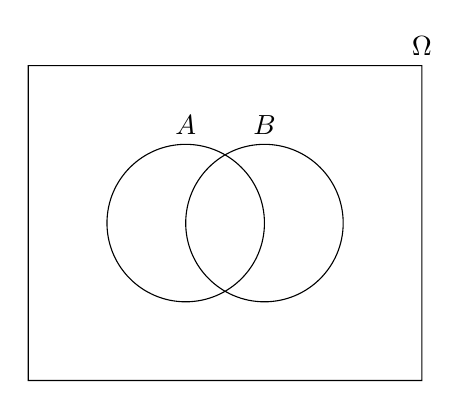
\begin{tikzpicture}[fill=white]
% left hand
\scope
\clip (-2,-2) rectangle (2,2)
      (1,0) circle (1);
\fill[white] (0,0) circle (1);
\endscope
% right hand
\scope
\clip (-2,-2) rectangle (2,2)
      (0,0) circle (1);
\fill[white] (1,0) circle (1);
\endscope
% outline
\draw (0,0) circle (1) (0,1)  node [text=black,above] {$A$}
      (1,0) circle (1) (1,1)  node [text=black,above] {$B$}
      (-2,-2) rectangle (3,2) node [text=black,above] {$\Omega$};
\end{tikzpicture} & &
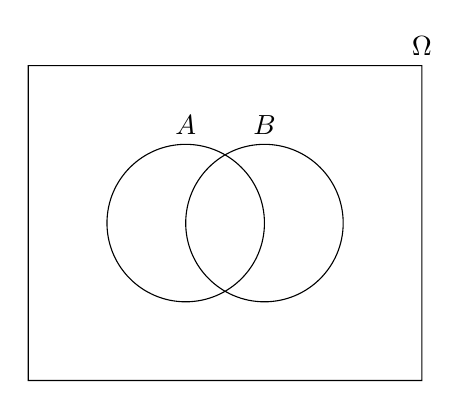
\begin{tikzpicture}[fill=white]
% left hand
\scope
\clip (-2,-2) rectangle (2,2)
      (1,0) circle (1);
\fill[white] (0,0) circle (1);
\endscope
% right hand
\scope
\clip (-2,-2) rectangle (2,2)
      (0,0) circle (1);
\fill[white] (1,0) circle (1);
\endscope
% outline
\draw (0,0) circle (1) (0,1)  node [text=black,above] {$A$}
      (1,0) circle (1) (1,1)  node [text=black,above] {$B$}
      (-2,-2) rectangle (3,2) node [text=black,above] {$\Omega$};
\end{tikzpicture} \\
 &  & \\
  &  & \\
(c) $A \cap B$ & & (d) $A-B$\\
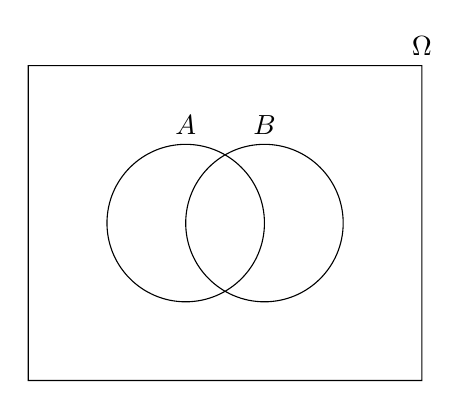
\begin{tikzpicture}[fill=white]
% left hand
\scope
\clip (-2,-2) rectangle (2,2)
      (1,0) circle (1);
\fill[white] (0,0) circle (1);
\endscope
% right hand
\scope
\clip (-2,-2) rectangle (2,2)
      (0,0) circle (1);
\fill[white] (1,0) circle (1);
\endscope
% outline
\draw (0,0) circle (1) (0,1)  node [text=black,above] {$A$}
      (1,0) circle (1) (1,1)  node [text=black,above] {$B$}
      (-2,-2) rectangle (3,2) node [text=black,above] {$\Omega$};
\end{tikzpicture} & &
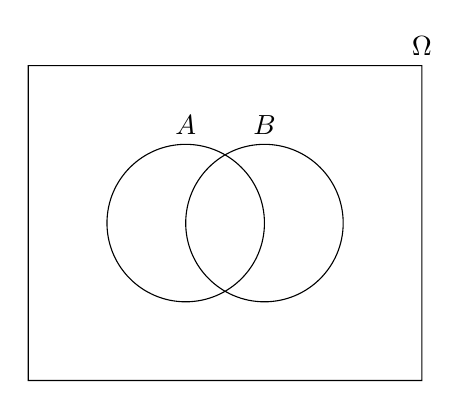
\begin{tikzpicture}[fill=white]
% left hand
\scope
\clip (-2,-2) rectangle (2,2)
      (1,0) circle (1);
\fill[white] (0,0) circle (1);
\endscope
% right hand
\scope
\clip (-2,-2) rectangle (2,2)
      (0,0) circle (1);
\fill[white] (1,0) circle (1);
\endscope
% outline
\draw (0,0) circle (1) (0,1)  node [text=black,above] {$A$}
      (1,0) circle (1) (1,1)  node [text=black,above] {$B$}
      (-2,-2) rectangle (3,2) node [text=black,above] {$\Omega$};
\end{tikzpicture}
\end{tabular}
\ee

%\clearpage

%\pagebegin{Important Venn Diagrams}


%\begin{center}
%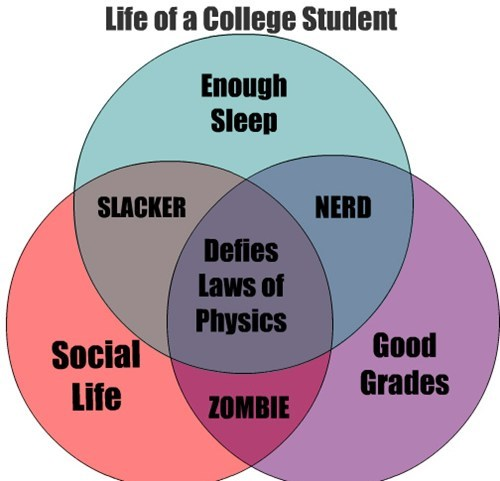
\includegraphics[width=3in]{03/03-venn_student.jpg} \ \ \ \ \ 
%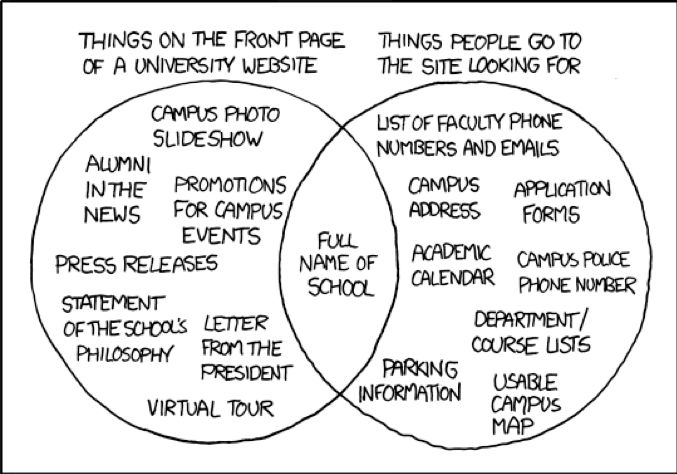
\includegraphics[width=3in]{03/03-web_venn.png}
%\end{center}

%\vspace{0.75in}

%\begin{center}
%\includegraphics[width=3in]{03/03-venn_drwho.jpg} \ \ \ \ \ \ 
%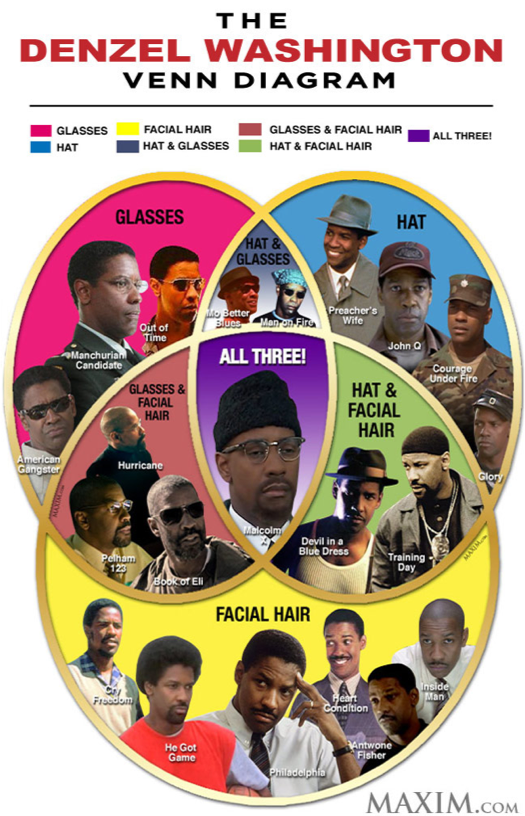
\includegraphics[width=2in]{03/03-denzel_venn.png}
%\end{center}


\clearpage
\pagebegin{Probability Rules}

We can generalize the calculations from the previous case study on vitamin A and childhood morbidity to obtain the following results:

\bbox
\begin{theorem}
Let $A$ and $B$ denote two events in sample space $\Omega$, then
\bi
\ii \textbf{\alert{Additive rule}}: $P(A \cup B) = P(A) + P(B) - P(A \cap B)$.
\ii \textbf{\alert{Bayes' Theorem}}: $\dsty P(B | A) = \frac{P(A \cap B)}{P(A)}$
\ii \textbf{\alert{Multiplicative rule}}: $P(A \cap B) = P(A) \cdot P(B | A)$
\ii \textbf{\alert{Complement rule}}: $P(A^C) = 1 - P(A)$
\ei
\end{theorem}
\ebox

\bb[resume] 
\ii When a customer purchases a new car, they are presented with a menu of options such as heated steering wheel, parking assistant, satellite radio, etc. The two most popular options on a certain type of new car are a sunroof (denoted $S$) and heated seats (denoted by $H$). Answer the following questions if we know that 
\[ P(S) = 0.6, \quad P(H) = 0.45,\mbox{ and} \quad P(H | S ) = 0.65 \] \label{q:cars}

\bb
\ii Interpret the practical meaning of $P(H | S ) = 0.65$. \vfill
\ii Compute $P(H^C)$ and interpret the meaning. \vfill
\ii Compute $P(S \cap H)$ and interpret the meaning. \vfill
\ii Compute $P(S | H)$ and interpret the meaning. \vfill
\ee
\ee

\clearpage

\pagebegin{Independent Events}

Often in statistics we want to investigate questions such as:
\bi
\ii Is a newly developed vaccine effective?
\ii Do certain sentencing laws have an effect on crime rates?
\ii Did increasing the minimum wage for fast food workers effect fast food prices?
\ii \textbf{Does the occurrence of one event (getting a sunroof) effect the likelihood that another event (heated seats) occurs?}
\ei

\bb[resume]
\ii In the car option example in question \ref{q:cars}, we know that  $P(S) = 0.6$, $P(H) = 0.45$, and $P(H | S ) = 0.65$. Based on this information, \textbf{if a customer has purchased the sunroof option, are they more, less, or equally likely to get the heated seats option?} Explain how you determined your answer.

\vfill


\ee

\bbox
\begin{definition}\label{def:ind}
Two events $A$ and $B$ are \textbf{\alert{independent}} if the occurrence of one has no effect on the occurrence of the other:

\vspace{0.5in}

%\[ P(B) = P(B | A) \quad \mbox{or} \quad P(A) = P(A | B), \]
\alert{Special case:} If events $A$ and $B$ are independent events then we have $P(A \cap B) = P(A)P(B)$.
\end{definition}
\ebox

\bb[resume]

\ii A person flips a fair coin and stops once they get at least one head and one tail. What is the probability that it takes exactly four flips to get exactly one head and one tail.

\vfill

\ee

\clearpage

%\ii Assume that the overall risk of breast cancer in a 45 year old woman is 1\%. The mammogram test used to screen for
%breast cancer is 90\% \textbf{sensitive}, meaning the test gives a correct positive 90\% of the time. We also know that the mammogram test is 95\% \textbf{specific}, meaning the test gives a correct negative 95\% of the time.\label{medical}
%%Let $D$ denote the event that a 45 year old woman has breast cancer (so $D^C$ is the event she is cancer free). Let $X$ denote the event that the mammogram result is positive for breast cancer (so $X^C$ is the event the screening comes back negative). 
%%\begin{multicols}{2}

%\begin{center}
%\begin{tabular}{c||c|c||c}
%\hline
%\  & $X$, Test Positive & $X^C$, Test negative & Total\\
%\hline
%\hline
%$D$, does have breast cancer &  &  & \\
%\hline
%$D^C$, does NOT have breast cancer &  &  & \\
%\hline
%\hline
%Total &  &  & $100$
%\end{tabular}
%\end{center}

%%\columnbreak
%\bb
%\ii For example, if 100 woman take a mammogram test, fill in the rest of the blanks to complete the \textbf{contingency table} above. \ss
%\ii Are events $D$ and $X$ independent? Show or explain why or why not? \vfill
%%\ee
%%\end{multicols}
%%\bb
%%\addtocounter{enumii}{2}
%\ii What is the probability that a randomly selected 45 year old woman has breast cancer and has a positive test result? \vfill
%\ii What is the probability that a randomly selected 45 year old woman has breast cancer or has a positive test result? \vfill
%\ii You are a doctor who has a 45 year old female patient whose mammogram result is positive. How likely is this patient
%to actually have breast cancer?\vfill
%\ee
%\ee

%\bb[resume]
%\ii According to Lord Mersey's original report to the British Parliament in 1912, there were a total of $2,\!224$ passengers and crew aboard the Titanic when it sank, resulting in the death of $1,\!513$ passengers and crew.  The \textbf{contingency} (or two-way) table shows the passenger breakdown. Let $A_1$, $A_2$, $A_3$ and $A_4$ be the event a randomly selected person onboard the Titanic is first-class, second-class, third-class or crew. Let $S$ be the event the passenger survived.

%\begin{multicols}{2}

%\begin{center}
%\begin{tabular}{c||c|c||c}
%\hline
%\  & Survived & Died & Total\\
%\hline
%\hline
%1st & 203 & 122 & 325\\
%\hline
%2nd & 118 & 167 & 285\\
%\hline
%3rd & 178 & 528 & 706\\
%\hline
%Crew & 212 & 696 & 908\\
%\hline
%\hline
%Total & 711 & 1,\!513 & 2,\!224
%\end{tabular}
%\end{center}

%\columnbreak

%\bb
%%\ii What is the probability that a randomly selected passenger on the Titanic survived?
%\ii Are events $A_2$ and $S$ independent? Show why or why not?
%\ee
%\end{multicols}
%\bb
%\addtocounter{enumii}{1}
%\ii What is the probability that a randomly selected passenger survived and was second-class? \vfill
%\ii What is the probability that a randomly selected passenger survived or was second-class? \vfill
%\ii What is the probability that a randomly selected passenger survived given that we know the passenger was second-class? \vfill
%\ii What is the probability that a randomly selected passenger was second-class class given that we know the passenger survived? \vfill
%\ee
%\ee

%\clearpage

%\pagebegin{Conditional Probabilities}

%\bb[resume]
%\ii Based on your work in \ref{medical}, fill in the blank in definition \ref{def:conditional} below.
%\ee

%\bbox
%\begin{definition}\label{def:conditional}
%If $P(B) >0$, then the \textbf{conditional probability} of $A$ given $B$ is denoted
%\[ P(A \mid B) = \rule{0.2\tw}{0.5pt}.\]
%\end{definition}
%\ebox

%\bb[resume]
%\ii Complete the lemma by filling each blank with one of the following: $P(A \mid B)$, $P(B \mid A)$, $P(A \cap B)$, $P(A)$, or $P(B)$.
%\begin{lemma}\label{lemma:conditional}
%From definition \ref{def:conditional} it follows that
%\bi
%\ii $P(A \cap B) = $ \rule{0.1\tw}{0.5pt} $\cdot P(B) = $ \rule{0.1\tw}{0.5pt} $\cdot P(A)$. \bs
%\ii If $A$ and $B$ are independent events, then $P(A \mid B) = $ \rule{0.1\tw}{0.5pt} .
%\ei
%\end{lemma}
%\ee


\clearpage

\pagebegin{Probability Distributions}

\bbox
\begin{definition}
Two events $A$ and $B$ are \textbf{disjoint} (or \textbf{mutually exclusive}) if they cannot occur at the same time, and therefore $P(A \cap B) = 0$.
\smallskip

\alert{Special case:} If events $A$ and $B$ are disjoint then we have $P(A \cup B) = P(A)+P(B)$.
\end{definition}
\ebox

%\bb[resume]
%\ii Returning to the job applicants example in \ref{applicants}, give an example of:\label{disjoint}
%\bb
%\ii Three different events that are disjoint from one another.\label{aredisjoint} \vfill
%\ii Two different events that are NOT disjoint from one another.\label{notdisjoint} \vfill
%\ee
%\ee


\bb[resume]
%\ii Do the three events you identified in \ref{aredisjoint} form a partition of the sample space $S$ in \ref{applicants}? Show or explain why or why not.
\ii In the options for a new car example in question \ref{q:cars}, are events $H$ and $S$ mutually exclusive? Why or why not? \vfill

\ee

\bbox
\begin{definition}\label{def:prob-dist}
A function $P$ that assigns a real number $P(A)$ to each event $A$ is a \textbf{probability distribution} or a \textbf{probability measure} if it satisfies the following three axioms:
\bb
\ii $P(A) \geq$ \rule{0.1\tw}{0.5pt} for all $A$. \bs
\ii $P(\mbox{full sample space})=P(\Omega) =$ \rule{0.1\tw}{0.5pt} . \bs
\ii If $A$ and $B$ are disjoint, then
\[ P \left( A \cup B \right) = \mbox{\rule{0.25\tw}{0.5pt}}.\]
\ee
\end{definition}
\ebox

%\bb[resume]
%\ii Prove that as a result of definition \ref{def:prob-dist} it follows that $P(A) = 1-P(A^C)$.'\vfill \vspace{1in}

%\ii A fair coin is tossed until we get exactly two heads. What is $\Omega$, the sample space? What is the subset, call it $A$, that corresponds to requiring exactly 4 tosses? What is $A^C$?

%\ee

\clearpage

\pagebegin{OPTIONAL: Counting}


\bb[resume]
\ii 5 people have volunteered to work on a committee. The committee will consist of a total of three people. How many different committees of 3 people can be formed from the 5 volunteers? \vfill
\ee


\bbox
We often need to count the number of ways of choosing $k$ items out of $n$ possible items. You may recall this is often called \textbf{$\mathbf{n}$ choose $\mathbf{k}$} and is denoted as

\[ \left( \begin{array}{c} n \\ k \end{array}\right) = \frac{n!}{k!(n-k)!}.\]
\ebox

\bb[resume]
\ii BONUS: Suppose $n$ people are in a room. What is the probability that there is at least one pair of people that have the same birthday? \textit{Hint: Let $A$ be the event there is no match. Calculate $P(A)$, and then find $P(A^C)$.} %\vfill

\vfill

\ee



%\clearpage

\begin{center}
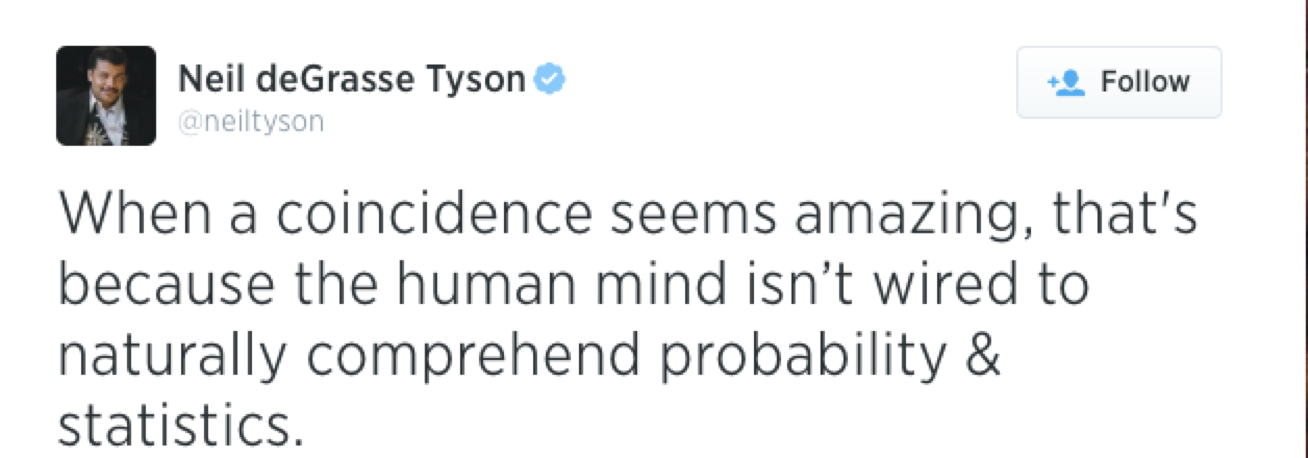
\includegraphics[width=5in]{03/tyson-tweet.png}
\end{center}
\bs

%\bbox
%\bi 
%\ii A \textbf{statistical experiment or observation} is any random activity that results in a definite outcome.
%\ii The \textbf{sample space} $\Omega$ is the set of all possible outcomes of an experiment.
%\ii An \textbf{outcome, realization or elements}, $\omega$, is a result from an experiment or observation.
%\ii An \textbf{event}, $A$, is a collection of one or more outcomes from an experiment or observation.
%\ei
%\ebox

%\bb
%\ii There are two people in a room. You ask each person what is their birthday (excluding the year).
%\bb
%\ii List several outcomes in the sample space. How many outcomes are in the sample space $\Omega$? \vfill
%\ii Let $M$ denote the event that the two people have the same birthday. How many outcomes are in this event? \vfill
%\ee

%\ii At the end of the semester I randomly select a student in the course and observe their average for the semester.
%\bb
%\ii What is the sample space $\Omega$? \vfill
%\ii What is the event that a student passes the course? \vfill
%\ee

%\ii If possible, give an example of an \textbf{infinite sample space} that is \textbf{discrete}? \vfill

%\ee


\clearpage

\pagebegin{OPTIONAL: Bayes' Theorem}

\bbox
\begin{definition}
A \textbf{partition} of a space $\Omega$ is a collection of disjoint sets such that $\dsty \bigcup_{i=1}^{\infty} A_i = \Omega$.
\end{definition}
\ebox



%%%%%%%%%%%%%%
%% Move elsewhere
%%%%%%%%%%%%%%
\bb[resume]

\ii Fill in the blank to complete theorem \ref{thm:total-prob} below and explain (in words, pictures, or equations) how you determined your answer.

\begin{multicols}{2}

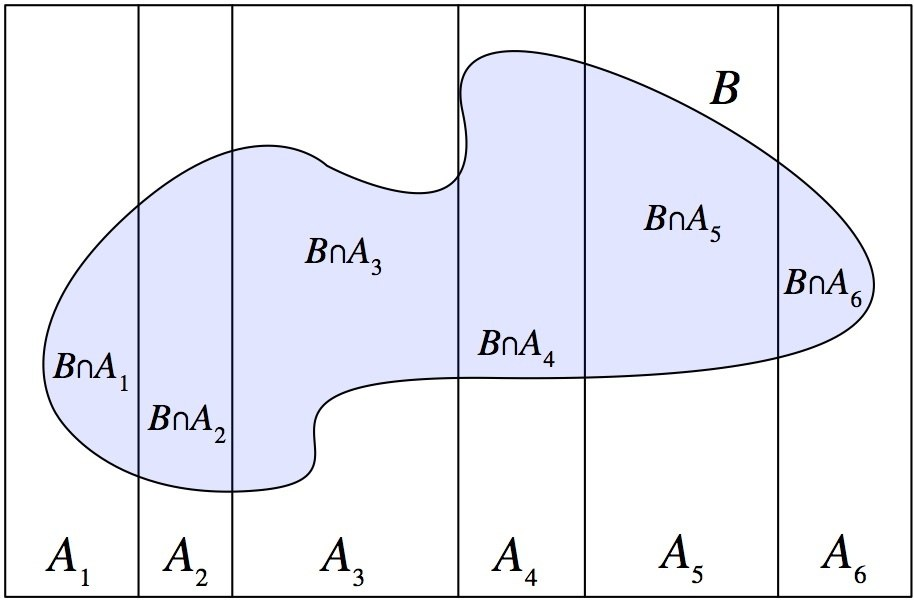
\includegraphics[width=0.4\tw]{03/03-venn-totalprob.jpg}

\columnbreak
\bbox
\begin{theorem}{Law of Total Probability}\label{thm:total-prob}
Let $A_1$, $A_2$, $\ldots , A_k$ be a partition of $\Omega$. Then for any event $B$,
\[ P(B) = \sum_{i=1}^k \rule{0.2\tw}{0.5pt}.\]
\end{theorem}
\ebox

\end{multicols}
\ee

%%%%%%%%%%%%%%
%% Move elsewhere
%%%%%%%%%%%%%%


\clearpage

\bbox
\begin{theorem}{Bayes' Theorem}\label{thm:bayes}
Let $A_1$, $A_2$, $\ldots , A_k$ be a partition of $\Omega$ such that $P(A_i)>0$ for each $i$. If $B$ is any event with $P(B)>0$, then for each $i=1, \ldots k$, we have
Then for any event $B$,
\[ P(A_i \mid B) = \frac{P(A_i \cap B) }{P(B)} = \frac{P(B \mid A_i) P(A_i)}{\sum_{j=1}^k P(B \mid A_j)P(A_j)}.\]
\end{theorem}
\ebox

\bb[resume]
\ii Suppose that 30\% of computers run Mac, 50\% use PC, and 20\% use Linux. A computer virus is
created by hackers, and suppose that  65\% of Mac, 82\% of PC, and 50\% of Linux computers get the virus.
\bb
\ii What is the probability that a randomly selected computer has the virus? \vfill
\ii What is the probability that a randomly selected computer is PC given that the computer is infected by the virus?\vfill \vspace{1in}
\ee
\ee

%\ii Recall the Monty Hall problem. Imagine you are playing the game and initially select door number 1. The game show host than opens one of the other doors (door 2 or door 3) to reveal one of the goats. Let $W$ denote the event the contest wins after making their decision (either \textit{Switch} or \textit{Stay}).
%\bb
%\ii Calculate $P(W \mid \mbox{\textit{Stay}})$. \vfill
%\ii Calculate $P(W \mid \mbox{\textit{Switch}})$. \vfill
%\ii What is the best strategy?  \vfill
%\ii Are $W$ and \textit{Stay} independent events? Mutually exclusive events? \vfill
%\ee
